\documentclass{article}
\usepackage[letterpaper, margin = 1 in]{geometry}
\usepackage{graphicx}
\graphicspath{.}
\usepackage{float}

\begin{document}

\noindent \textbf{Flat Plate} \\ \\
Vortex of strength $\Gamma$ = -0.02 started upstream at (-4.5,0.04). Graph below shows comparison of obtained results to the analytical lift response of a flat plate to a passing vortex. Note that the lift for both analytical and numerical results have been `normalized' by the strength of the vortex $\Gamma$.\\
\begin{equation}
L = \rho \Gamma \frac{c}{2} e^{-kh} \big(-i S\big(k \big) \big)
\end{equation}

\begin{figure}[h]
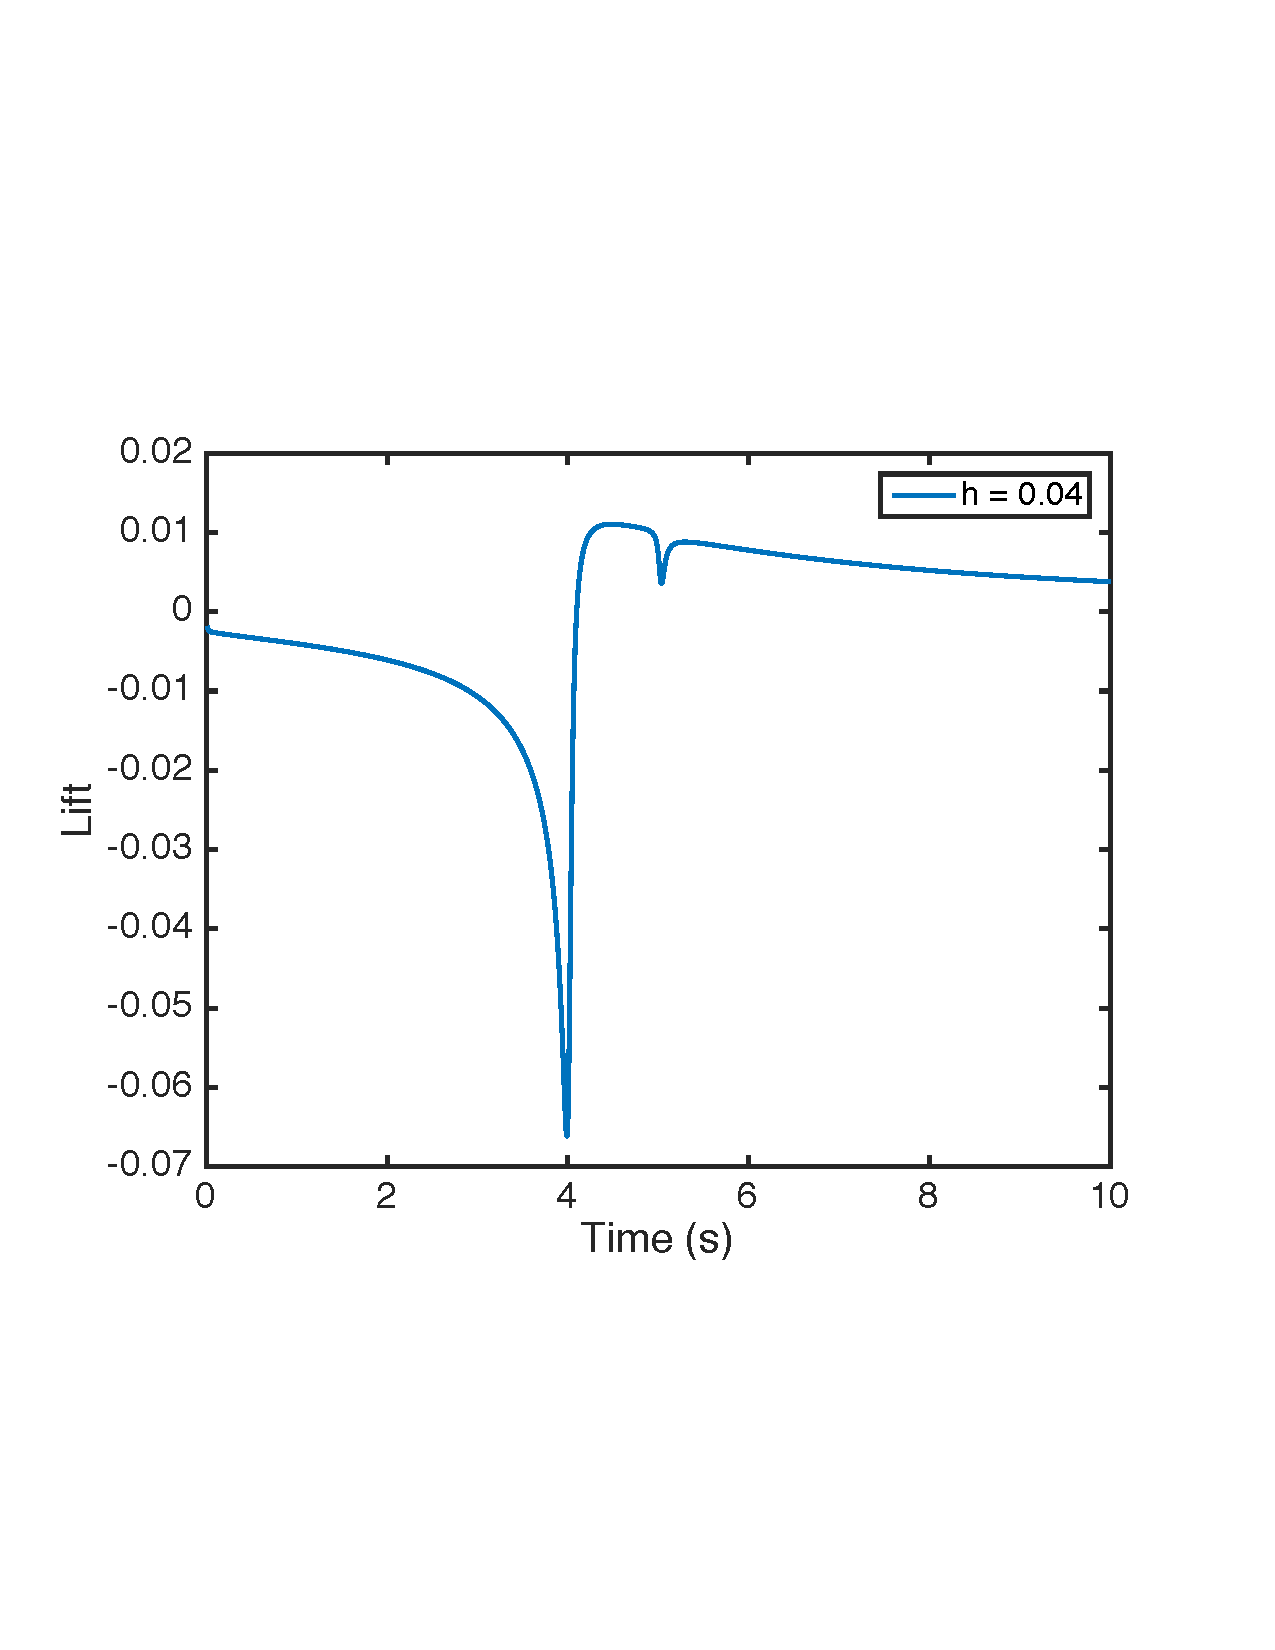
\includegraphics[width = 4 in, height = 3 in]{Lift_Curve}
\centering
\caption{Lift Curve Response of Flat Plate to Passing Vortex}
\end{figure}

\begin{figure}[h]
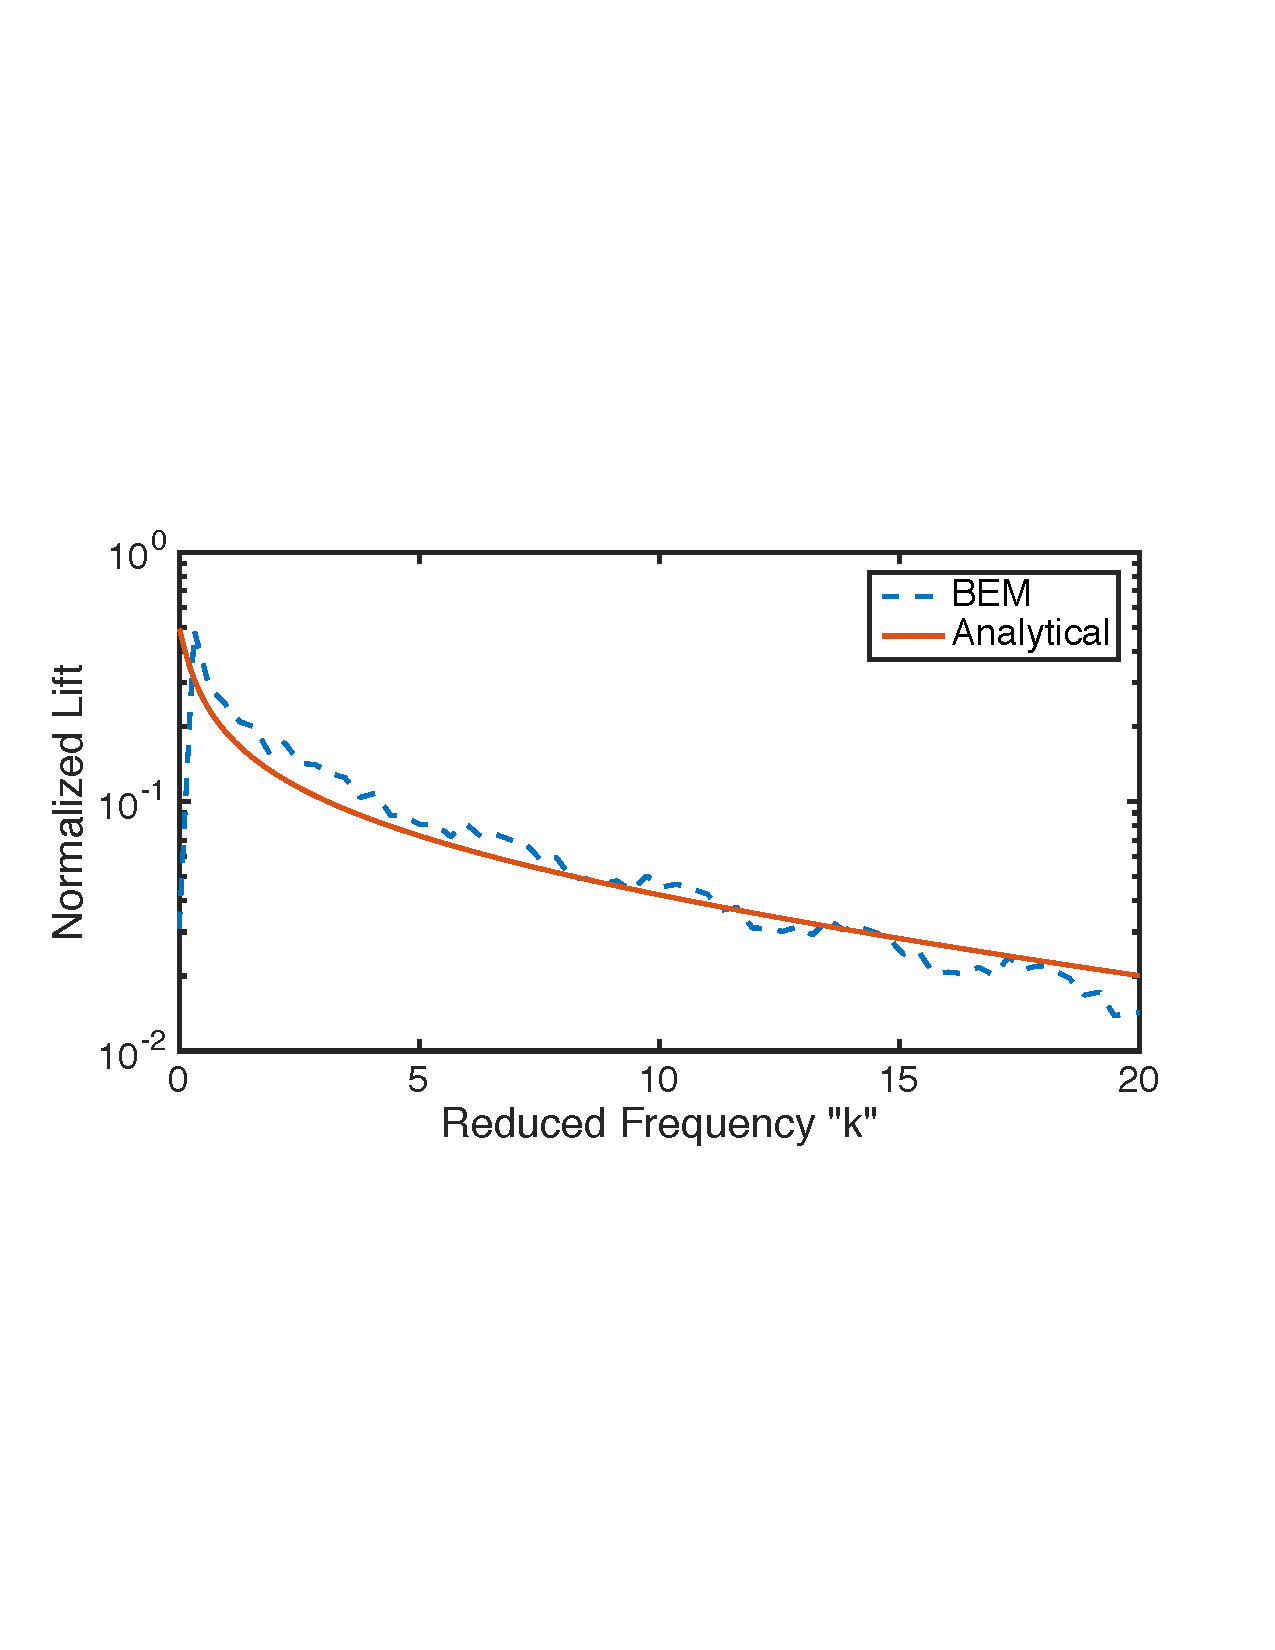
\includegraphics[width = 4 in, height = 3 in]{SearsVsBEM}
\centering
\caption{Analytical and BEM Spectrum of Lift for Vortex Passing Flat Plate}
\end{figure}
\newpage

%\begin{figure}[h]
%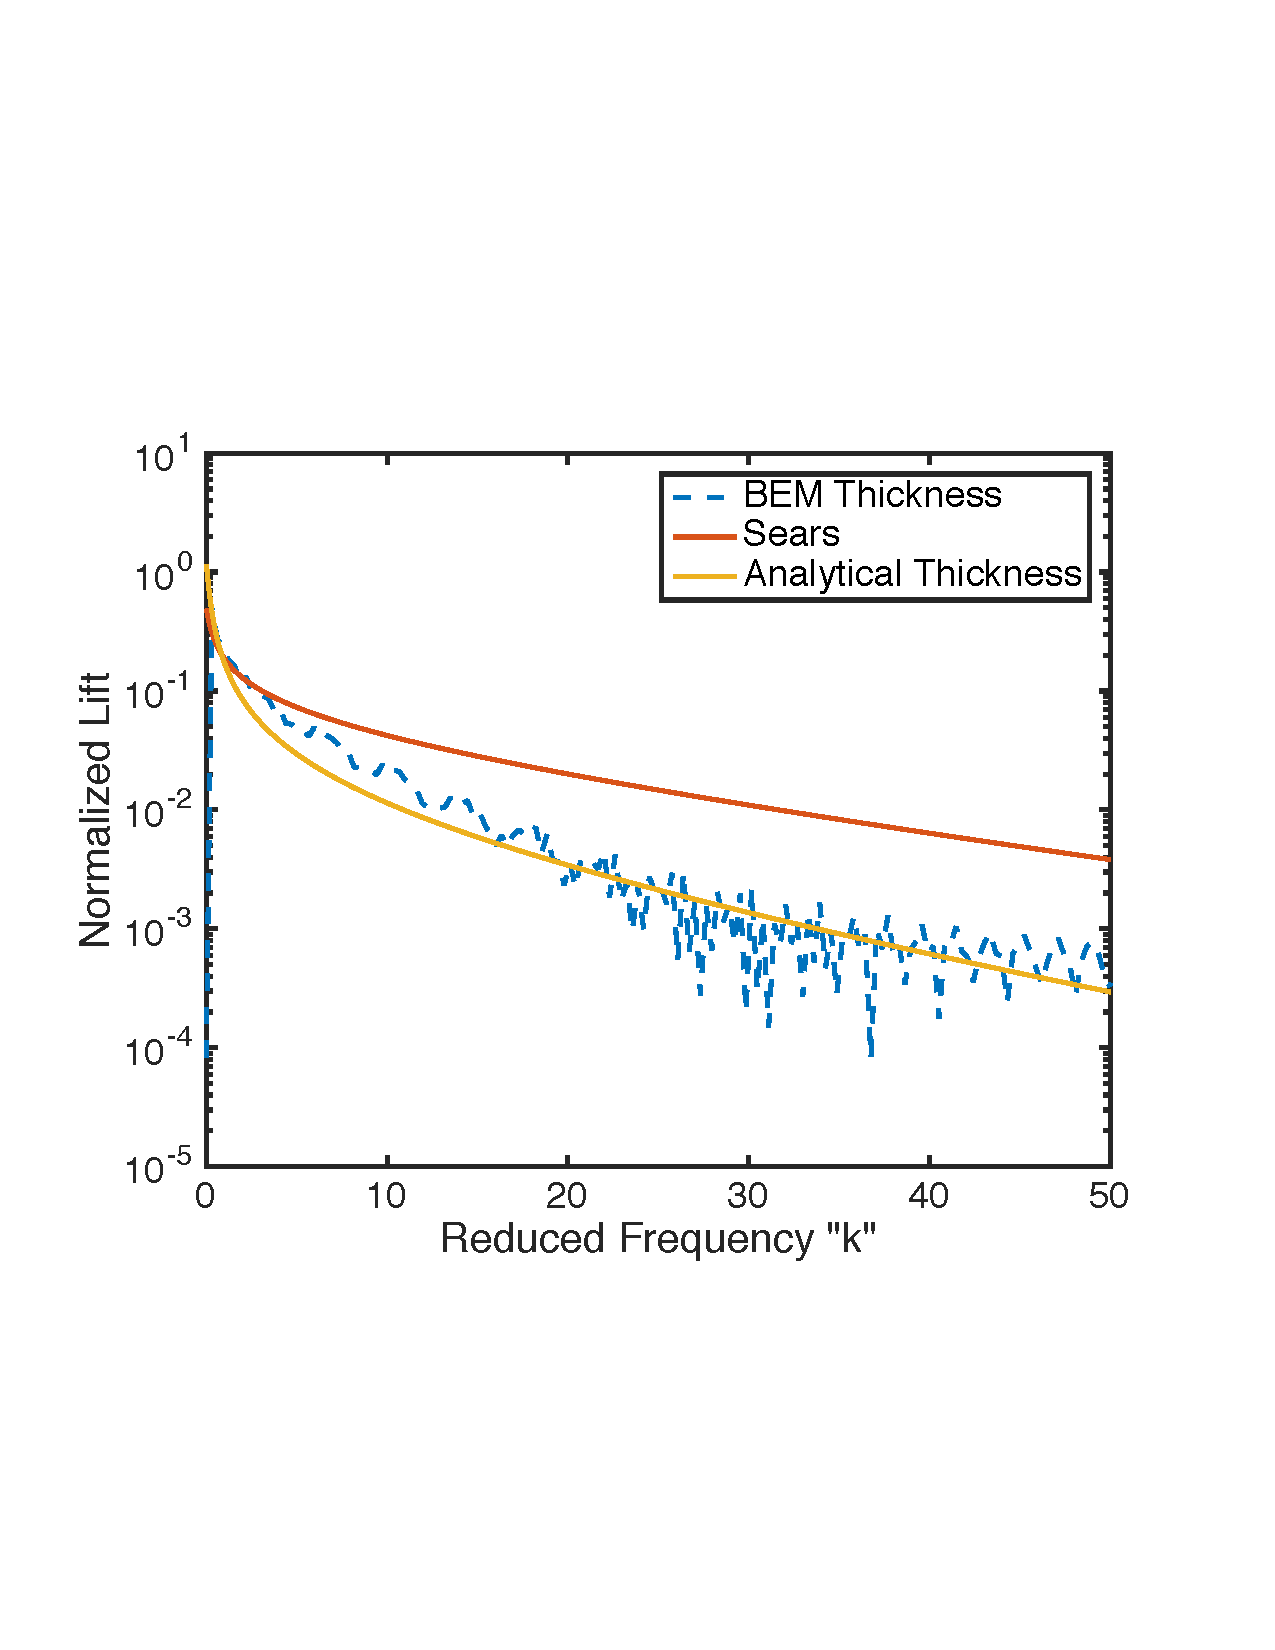
\includegraphics[width = 4 in, height = 3 in]{BEM_Compare}
%\centering
%\caption{Comparison of Lift Spectrums}
%\end{figure}

\end{document}


